\section{Approach}
\label{sec:approach}

MAM accepts a set of projects as data sources for mining API
mapping relations between two languages $L_1$ and $L_2$. 
For each project used as a data source,
MAM requires at least two versions of the project (one
version in $L_1$ and the other version in $L_2$).
Figure~\ref{fig:approach} shows the overview of MAM.

First, MAM aligns client code in languages $L_1$ and $L_2$
so that the aligned source files implement similar functionalities
(Section~\ref{sec:approach:acc}). Second, MAM mines
mapping relations of API classes (Section~\ref{sec:approach:mappingtypes}).
Finally, MAM mines mapping relations of API
methods (Section~\ref{sec:approach:mappingmethods}) defined by the mapped
API classes.

\begin{figure}[t]
\centering
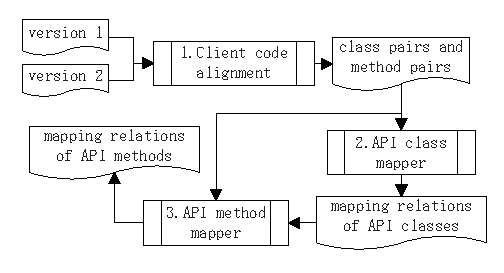
\includegraphics[scale=1,clip]{figure/approach.eps}\vspace*{-3ex}
 \caption{Overview of MAM}\vspace*{-3.5ex}
 \label{fig:approach}
\end{figure}

%-------------------------------------------------------------------
\subsection{Aligning API Client Code}
\label{sec:approach:acc}

Initially, MAM accepts two versions of a project (one version in
$L_1$ and the other version in $L_2$) and aligns classes and methods
of the two versions. Aligned classes or methods
between the two versions implement a similar functionality. As they
implement a similar functionality, APIs used by these classes or methods can be
replaceable.

To align classes and methods of the two versions, MAM uses
name similarities between entities (such as class names or method
names) defined by the two versions of the project. In MAM,
we have two different kinds of entity names: entity names defined by
the two versions of the project and entity names of third-party
libraries used by the two versions of the project. The first kind
often comes from the same programmer or the same team, or
programmers may refer to existing versions for naming entities such
as classes, methods, and variables. Therefore, name similarity of
the first kind is often reliable to distinguish functionalities
compared to the second kind. MAM uses
Simmetrics\footnote{\url{http://sourceforge.net/projects/simmetrics/}}
to calculate name similarities.

We next describe how MAM aligns client-code classes.
The first step is to find candidate class pairs by names. For two sets
of classes $C$ and $C'$, MAM returns candidate class
pairs $M$ with a similarity greater than a given threshold,
referred to as \emph{SIM\_THRES- HOLD}. As some projects may have more
than one class with the same name, $M$ may contain more than one
mapping pair for a class in a version. To align those classes, MAM uses package names of these classes to refine $M$ and
returns only one mapping pair with the maximum
similarity\footnote{For C\#, we refer to namespace names for package
names.}.

In each aligned class pair, MAM further aligns methods
within the class pair. The algorithm for methods is similar to the
algorithm for classes and also may return more than one candidate
method pair due to overloading. Here, the algorithm for methods
relies on criteria such as the number of parameters and names of
parameters to refine candidate method pairs. For the example shown
in Section~\ref{sec:example}, MAM correctly aligns the
class \CodeIn{IndexFiles} and the method \CodeIn{main} in Java to
the class \CodeIn{IndexFiles} and the method \CodeIn{Main} in C\#,
respectively, as their names are quite similar.
%-----------------------------------------------------------------
\subsection{Mapping API classes}
\label{sec:approach:mappingtypes}

In this step, MAM mines mapping relations of
API classes. As mapping relations of API classes are used
to translate variables, MAM mines mapping
relations of API classes based on how aligned client code declares
variables such as fields of aligned classes, parameters, and local variables of aligned methods. For each aligned class pair $\Pair{c_1} {c_2}$, MAM analyzes each field pair $\Pair{f_1}{f_2}$ and considers
$\Pair{f_1.type} {f_2.type}$ as a relation, if the similarity between $f_1.name$ and $f_2.name$ is
greater than \emph{SIM\_THRESHOLD}. Similarly, for each aligned method pair
$\Pair{m_1} {m_2}$, MAM analyzes each local variable pair
$\Pair{v_1} {v_2}$ and considers $\langle v_1.type,$ $
v_2.type\rangle$ as a relation, if the similarity between
$v_1.name$ and $v_2.name$ is greater than
\emph{SIM\_THRESHOLD}. Also, MAM analyzes each parameter pair
$\langle p_1, p_2\rangle$ of $m_1$ and $m_2$, and MAM considers $\langle p_1.type, p_2.type\rangle$ as
a relation when the similarity between $p_1.name$ and $p_2.name$ is greater than \emph{SIM\_THRESHOLD}.

For the example shown in Figure~\ref{fig:clientcode}, MAM
mines the mapping relation between \CodeIn{java.io.File} and
\CodeIn{System.IO.FileInfo} based on the mapped fields of Lines 6
and 11. The mapping relation of API
classes helps translate the variable declared in Line 1
(Figure~\ref{fig:challenge}) to the variable declared in Line 3
(Figure~\ref{fig:challenge}).

%\begin{algorithm}[t]
%\begin{SmallOut}
%\dontprintsemicolon
%  \KwIn{$C$ is the classes of a language; $C'$ is the classes
%  of another language}
%  \KwOut{$P$ is aligned pairs of classes}
%  \Begin{
%     $M \leftarrow findCandidateClassPairs(C, C')$\;
%     \While{$M.size > 0 $}{
%        \If{$M.size > 1$}{
%            $M \leftarrow refineByPackageNames(M)$\;
%         }
%         \If{$M.size == 1$}{
%                $P.add(M)$\;
%                $C.remove(M[0].c)$\;
%                $C'.remove(M[0].c')$\;
%         }
%         $M \leftarrow findCandidateClassPairs(C, C')$\;
%     }
% }
%\end{SmallOut}
%\label{alg:alignclasses} \caption{Align Classes Algorithm}
%\end{algorithm}

%\begin{figure}[t]
%\centering
%\includegraphics[scale=1,clip]{figure/algorithm1.eps}
%\vspace*{-6ex}
%\end{figure}

%-----------------------------------------------------------
\subsection{Mapping API methods}
\label{sec:approach:mappingmethods}

In this step, MAM mines mapping relations of API methods.
This step has two major sub-steps. First, MAM builds a graph, referred
to as API transformation graph, for each client code
method. Second, MAM compares the two graphs of each pair of
client-code methods for mining mapping relations of API methods.

\begin{figure*}[t]
\centering
\includegraphics[scale=1.1,clip]{figure/graph.eps}\vspace*{-3ex}
 \caption
{\label{fig:graph}Built ATGs and the main steps of comparing
ATGs}\vspace*{-3.5ex}
\end{figure*}

%-------------------------------------------------------------
\subsubsection{API Transformation Graph}

We propose API Transformation Graphs (ATGs) to help deal with two
major challenges. (1) Mapping parameters of an API method in one language with
parameters of an API method in the other language can be complex. (2) An API
method of one language can be mapped to more than one API method in the
other language.

An ATG of a client-code method $m$ is a directed graph $G\langle N_{data},$ $ N_m, E\rangle$.
$N_{data}$ is a set of the fields $F$ of $m$'s declaring class, local variables $V$ of
$m$, parameters $P_1$ of $m$, parameters $P_2$ of API methods invoked
by $m$, and returns $R$ of all methods. $N_{m}$ is a set of
methods invoked by $m$. $E$ is a set of directed edges. An edge
$d_1\rightarrow d_2$ from a datum $d_1 \in N_{data}$ to a datum $d_2
\in N_{data}$ denotes that $d_2$ is data-dependent on $d_1$, referred to as
data dependency from $d_1$ to $d_2$. An edge $d_1 \rightarrow m_1$ from a datum $d_1 \in N_{data}$ to a
method $ m_1 \in N_{m}$ denotes that $d_1$ is a parameter or receiver
of $m_1$. An edge $m_1 \rightarrow d_1$ from a method $m_1
\in N_{m}$ to a datum $d_1 \in N_{data}$ denotes that $d_1$ is the return
of $m_1$.

%We propose ATG for two main purposes. The first purpose is to mine mapping
%relations among parameters of mapped API methods. Mining mapping relations
%among parameters of mapped API methods is challenging as often mapped API methods
%can have different number of parameters or different positions among
%parameters. For example, consider the following two mapped API methods:
%
%\begin{CodeOut}
%$m_1$ in Java: BigDecimal java.math.BigDecimal.multiply (BigDecimal $p_1^1$)\\
%\hspace*{0.11in}$m_2$ in C\#: Decimal System.Decimal.Multiply (Decimal $p_1^2$, Decimal $p_2^2$)
%\end{CodeOut}
%
%Method $m_1$ of Java has a receiver variable, say $v_1^1$, of type \CodeIn{BigDecimal}
%and has one parameter $p_1^1$. The mapped method $m_2$ in C\# has
%two parameters $p_1^2$ and $p_2^2$. Using ATGs, MAM
%identifies that $v_1^1$ is mapped to $p_1^2$ and $p_1^1$ is mapped
%to $p_2^2$. As ATG captures parameters of API methods,
%MAM is able to deal with the challenges of mapping parameters.
%
%The second purpose of ATG is to mine mapping relations of merged API methods. As ATG
%describes data dependencies among inputs and outputs, MAM
%is able to mine mapping relations for merged API methods as shown in
%Figure~\ref{fig:example}. We next describe how MAM builds ATGs and
%uses ATGs for mining mapping relations of API methods.

%------------------------------------------------------------------
\subsubsection{Building API Transformation Graphs}

MAM builds an ATG for each method $m$ in the client code.
ATG includes information such as inputs
and outputs for each client-code method. In particular, for
each method $m$, MAM first builds subgraphs for its variables,
API methods, and field accesses. MAM adds additional edges
to the built ATG (and sub-graphs inside ATG) representing
data dependencies among built sub-graphs.
We use two notations for representing nodes in the ATG. A rectangle
represents a method labeled with the method name, whereas an ellipse
represents a datum such as fields, local variables, and parameters.
An ellipse is labeled as ``\emph{n:t}'', where \emph{n} is the name
of the variable and \emph{t} is its type. We use the
following rules for adding nodes and edges to the ATG.

\Comment{In particular, MAM analyzes source files of a
client code method statement by statement and adds edges according
to the rules as follows:}

%First, programming languages typically provide a huge set of APIs,
%and it is difficult to build mapping relations for all APIs
%manually. Second, some API methods have multiple parameters, and
%some parameters cannot be mapped directly one by one in orders. For
%example, \CodeIn{org.w3c.dom.Element.getAttributeNS()} and
%\CodeIn{System.Xml.XmlElement.GetAttribute()} both have two
%parameters, but the two parameters are inverse by their meanings.
%Third, one API method in one language may be mapped to more than one
%API method in other languages. For example, \CodeIn{java.util.
%LinkedList.removeLast()} returns the last value, and \CodeIn{System.
%Collections.Generic.LinkedList.RemoveLast()} does not return any
%values. To get that value, C\# programmers need to call more APIs,
%and thus one API method of Java is mapped to serval API methods of
%C\#.

%
%One challenge to mine mapping relations of two API methods lies in
%how to map their inputs correctly. Here, MAM both the
%receiver and the parameters of a method as the inputs of a
%method. Inputs of two API methods may be matched but are not in the
%same order. For example, as shown in Section~\ref{sec:example},
%\CodeIn{java.io. File.exist()} has a receiver whereas
%\CodeIn{System.IO.File.Exist()} has no receiver but a
%parameter. In addition, parameter orders may be quite different. For
%example, the parameter order of \CodeIn{org.w3c.
%dom.Element.getAttributeNS()} is inverse with the parameter order of
%\CodeIn{System.Xml.XmlElement.GetAttribute()}. To deal with the
%preceding problem,

\begin{enumerate}\vspace*{-2ex}
\item $\forall$ $f \in F \cup V \cup P_1$, MAM adds a node to the built ATG.
The reason for considering these variables such as fields in
the declaring class or local variables in method $m$ used in client code
is that these variables are useful to analyze data dependencies
among API methods.\vspace*{-2ex}
%\begin{center}
%\includegraphics[scale=0.7,clip]{figure/rule1.eps}
%\end{center}
\item $\forall$ API methods of the form ``$T_0\ T.AM (T_1 p_1, \ldots, T_n p_n)$''
invoked by method $m$, MAM adds a receiver node (of type $T$) and
parameter nodes to the built ATG as shown below. MAM does
not add a receiver node for static API methods. \vspace*{-2ex}

\begin{center}
\includegraphics[scale=0.7,clip]{figure/rule2.eps}%\vspace*{-1.5ex}
\end{center}\vspace*{-3ex}

\item $\forall$ $f\in F \cup V$, if $f$ is a non-primitive variable
of type $T_1$ and a field $x$ of $T_1$ is accessed as $f.x$, MAM adds nodes to the built ATG as shown below. As Java often
uses getters and setters whereas C\# often use field accesses, MAM treats field accesses as a special type of method
calls.\vspace*{-2ex}

\begin{center}
\includegraphics[scale=0.7,clip]{figure/rule3.eps}%\vspace*{-1.5ex}
\end{center}\vspace*{-3ex}

\item $\forall$ statements of the form $x = y$, where $x \in F \cup V \wedge y \in F \cup V$,
MAM adds an edge from $y$ to $x$. This edge represents that
$x$ is data-dependent on $y$.\vspace*{-1.5ex}

\begin{center}
\includegraphics[scale=0.7,clip]{figure/rule4.eps}%\vspace*{-1.5ex}
\end{center}\vspace*{-1.5ex}

\item $\forall$ statements of the form $x = AM()$, where $x \in F \cup V$, MAM
adds an edge from $AM$ to $x$ if the return of $AM$ is
assigned to $x$. This edge represents that $x$ is data-dependent on
the return of $AM$. \vspace*{-1.5ex}

\begin{center}
\includegraphics[scale=0.7,clip]{figure/rule5.eps}%\vspace*{-1.5ex}
\end{center}\vspace*{-1.5ex}

\item $\forall$ API methods $AM(x)$ invoked by method $m$, MAM
adds an edge from $x$ to the parameter node of $AM$. This edge
represents that the parameter of $AM$ is data-dependent on
$x$.\vspace*{-1.5ex}

\begin{center}
\includegraphics[scale=0.7,clip]{figure/rule6.eps}%\vspace*{-1.5ex}
\end{center}\vspace*{-1.5ex}

\item $\forall$ statements of the form $m_2(m_1(x))$, MAM
adds an edge from the return node of $m_1$ to the parameter
node of $m_2$ parameter node. This edge represents that the
parameter of $m_2$ is data-dependent on the return of $m_1$.\vspace*{-1.5ex}

\begin{center}
\includegraphics[scale=0.7,clip]{figure/rule7.eps}%\vspace*{-1.5ex}
\end{center}\vspace*{-1.5ex}

\item $\forall$ statements of the form $x.m()$, MAM adds
an edge from $x$ to $m$ since $x$ is the receiver of $m$. This
edge represents that the receiver of $m$ is data-dependent on
$x$.\vspace*{-1.5ex}

\begin{center}
\includegraphics[scale=0.7,clip]{figure/rule8.eps}%\vspace*{-1.5ex}
\end{center}\vspace*{-1.5ex}

\item $\forall$ statements of the form $ x = y\ op\ z\ op\ \ldots, op \in \{+,-,*,/\}$,
MAM adds edges from $y$, $z$, and others to $x$, since these
variables are connected by binary operations and the return is
assigned to $x$. The edge denotes the data dependency from $y$, $z$,
and other variables to $x$. For simplicity, MAM ignores
\emph{op} info. We discuss the issue in
Section~\ref{sec:discuss}.\vspace*{-1.5ex}
\begin{center}
\includegraphics[scale=0.7,clip]{figure/rule9.eps}%\vspace*{-1.5ex}
\end{center}\vspace*{-2ex}
\end{enumerate}

For each method $m$ in the client code, MAM applies the preceding
rules for each statement from the beginning to the end of $m$.
Within each statement, MAM applies these rules based on
their nesting depth in the abstract syntax tree. For example,
for the statements of the form $m_2(m_1(x))$, MAM first applies
these rules on $m_1$ and then on $m_2$.

Figures~\ref{fig:graph}a and ~\ref{fig:graph}b show partial ATGs for
C\# (\CodeIn{IndexFiles.cs}) and Java (\CodeIn{IndexFiles.java})
code examples shown in Figure~\ref{fig:clientcode}, respectively.
Figure~\ref{fig:graph} also shows corresponding line numbers of each
sub-graph. MAM applies Rules 2 and 8 for Lines 6 and 9
(Figure~\ref{fig:clientcode}) to build corresponding sub-graphs in
the ATG. MAM applies Rules 2, 3, and 6 to build corresponding
sub-graphs for Lines 11 and 14 (Figure~\ref{fig:clientcode}).

%\begin{algorithm}[t]
%\begin{SmallOut}
%\label{alg:mapATG} \dontprintsemicolon
%  \KwIn{$G$ is the ATG of a method ($m$); $G'$ is the ATG of $m$'s mapped method.}
%  \KwOut{$S$ is a set of mapping relations for API methods}
%  \Begin{
%     $P \leftarrow findVarPairs(m, m')$\;
%     \For{Pair p in P}{
%        $JM \leftarrow G.nextMethods(p.j)$\;
%        $SM \leftarrow G'.nextMethods(p.s)$\;
%        $\Delta S = mapping(SM, JM)$\;
%        \While{$\Delta S \neq \phi| \Delta SM \neq \phi| \Delta JM \neq \phi$}{
%            $S.addAll(\Delta S)$\;
%             \For{Method jm in JM}{
%                 \If{$jm.isMapped$}{
%                    $JM.replace(jm, jm.nextMethod())$\;
%                  }\Else{
%                    $JM.replace(jm, jm.mergeNextMethod())$\;
%                  }
%             }
%             $\Delta S = mapping(SM, JM)$\;
%             \For{Method sm in SM}{
%                 \If{$sm.isMapped$}{
%                    $SM.replace(sm, sm.nextMethod())$\;
%                  }\Else{
%                    $SM.replace(sm, sm.mergeNextMethod())$\;
%                  }
%             }
%        }
%     }
% }
% \end{SmallOut}
%\caption{ATG Comparison Algorithm}
%\end{algorithm}

\begin{figure}[t]
\centering
\includegraphics[scale=1,clip]{figure/algorithm2.eps}
\vspace*{-7ex}
\end{figure}

%--------------------------------------------------------------------
\subsubsection{Comparing API transformation graphs}

The second sub-step compares each pair of built ATGs for mining
mapping relations of API methods. Our mapped API methods should satisfy
three criteria. (1) The mapped API methods implement the same
functionality. (2) The mapping relation describes the relation between
parameters and receivers of mapped API methods. (3) The mapping relation
describes the relation between return of mapped API methods.
The two mapped API methods in two different languages satisfying the
preceding three criteria are replaceable in the client code.
Therefore, these mapped API methods assist for translating client
code from one language to another.

Algorithm 1 presents major steps of comparing ATGs for mining
mapping relations of API methods. For each pair of aligned methods $m$ and $m'$, the \CodeIn{findVarPairs} function finds mapped variables and constants as follows. For two variables $v$ and $v'$ $\in$ $F$, $V$, and $P_1$ in $m$ and $m'$, respectively,
\CodeIn{findVarPairs} maps $v$ and $v'$, if the similarity metric value on their names is greater
than \emph{SIM\_THRESHOLD}. For constants in $m$ and $m'$, \CodeIn{findVarPairs}
maps those two constants, if they have exactly the same
value. From matched variables and constants, our algorithm uses the following criteria to find mapping relations between two API methods $jm$ and $sm$.

\emph{Mapped inputs}: The first criterion is based on the inputs
of $jm$ and $sm$. We map $jm$ with $sm$, if there is a one-to-one
mapping between inputs of $jm$ and $sm$. Here, MAM
considers both the receiver and the parameters as the inputs of an
API method.

\emph{Mapped functionalities}: The second criterion is based on functionalities of
$jm$ and $sm$. We consider that $jm$ and $sm$ implement the same functionality,
if the similarity metric value between the name of $jm$ and the name of $sm$ is
greater than \emph{SIM\_THRESHOLD}.

\emph{Mapped outputs:} The third criterion is based on the returns of $jm$ and $sm$.
Consider the returns of $jm$ and $sm$ as $r_1$ and $r_2$, respectively. We map $jm$
with $sm$, if the type of $r_1$ is mapped with the type of $r_2$ in
mapping relations of API classes.

Our algorithm first attempts to map the first API method $jm$ in $m$
with the first API method $sm$ in $m'$. Our algorithm uses the \CodeIn{nextMethods}
function to get these $jm$ and $sm$ API methods. If our algorithm successfully maps $jm$ with
$sm$, our algorithm moves to the next available API methods in $m$
and $m'$ of the client code. If our algorithm is not able to map $jm$
with $sm$, our algorithm merges $sm$ and $jm$ with their next available API methods
in the corresponding ATGs, respectively, and attempts to map merged API methods.
Our algorithm uses the \CodeIn{replace} function for merging an API method with its
next available API method. For two merged API methods, our algorithm uses the
maximum similarity of method names between $jm$ and $sm$ as a
similarity metric value for mapping their functionalities.
With each iteration, $sm$ or $jm$ or the mapping relation (represented as $S$)
in the algorithm may change. Therefore, we repeat our algorithm
till $S$, $sm$, and $jm$ do not change anymore.

We next explain our algorithm using the illustrative example shown
in Figure~\ref{fig:graph}. The numbers shown in circles
represent the major steps in our algorithm for mining mapping
relations of API methods. We next explain each step in detail.

\emph{Step 1: mapping parameters, fields, local variables, and constants.}
Given two ATGs of each method pair $\langle m, m' \rangle$, this step maps
variables such as parameters, fields, and local variables by comparing their names,
and maps constants by comparing their values. As shown in
Figure~\ref{fig:graph}, Step 1 maps two constants since both the constants
have the same value ``\CodeIn{index}''.

\emph{Step 2: mapping inputs of API methods.} Step 2 mines mapping
relations of API methods using variable and constant mapping relations.
Initially, this step identifies the first API methods in the two ATGs and tries to
map their receiver and parameters of the two API methods.
In our current example, this step maps the parameter \CodeIn{filename}
to the parameter \CodeIn{arg0} as these parameters
are of the same type and their associated constants are mapped.

\emph{Step 3: mapping outputs of API methods.} In contrast to Step 2
that maps parameters, Step 3 maps returns of API methods. In
this step, if MAM is not able to map returns, MAM merges the next API method (Section~\ref{sec:mapping}) and
then attempts to map returns of merged API methods. In our current example shown in
Figure~\ref{fig:graph}, the return of \CodeIn{System.IO.FileInfo.FileInfo()}
cannot be mapped to the return of \CodeIn{java.io.File.File()}. Therefore, MAM merges subsequent API methods in the ATG till the \CodeIn{Exists}
API method, since the returns (shown as \CodeIn{Boolean}) can be mapped
only after the \CodeIn{Exists} API method. Figure~\ref{fig:graph}
shows Step 3 along with the mapped returns.

\emph{Step 4: mapping functionalities.} After MAM maps
parameters and returns, this step further maps functionalities
of those merged API methods. Given two merged API methods with
mapped parameters and returns, this step uses the similarity
metric value based on their method names as a criterion for mapping
their functionalities. In the preceding example, this step maps the
two merged API methods shown in Figure~\ref{fig:graph}a to the
merged API methods of the \CodeIn{java.io.File.exists()} as all
three merged API methods include the method named \CodeIn{exists}.

MAM applies the preceding steps on ATGs (as shown in
Figures~\ref{fig:graph}a and~\ref{fig:graph}b). After finding out
the mapped pair of API methods as shown in Figure~\ref{fig:graph},
MAM merges all variables and outputs to corresponding
parameters and receivers and produces the mapping relation of API
method as shown in Figure~\ref{fig:example}.
